\section{Pattern Analysis}

\begin{frame}{Pattern Analysis with EOF}
  \begin{columns}
    \begin{column}{.5\textwidth}
      \begin{itemize}
        \item \textit{very} closely related to PCA 
        \item widely used in geospatial sciences (see review paper from \citeauthor{hannachi_empirical_2007} \cite{hannachi_empirical_2007})
        \item can be used for dimensionality reduction, pattern recognition \dots
        \item applied to IVT fields \cite{ayantobo_integrated_2022, salstein_modes_1983, jiang_water_2009}
%        \item also some interesting modifications: REOFs
        \item \textbf{Plan}: Apply a similar windowed approach as \citeauthor{vietinghoff_visual_2021}
      \end{itemize} 
      
    \end{column}
    \begin{column}{.5\textwidth}
    \begin{figure}[t]
      \centering
      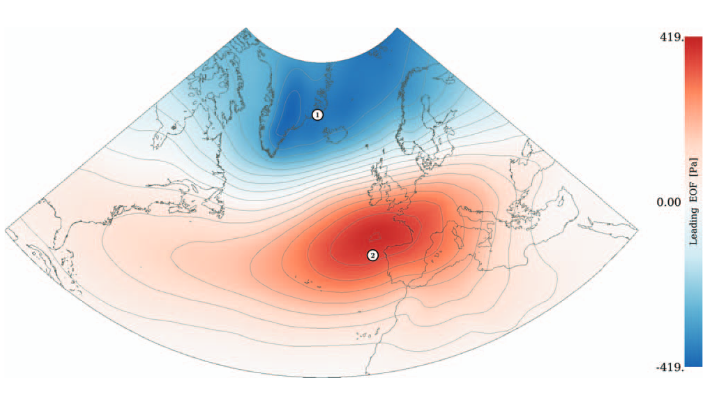
\includegraphics[width=.7\columnwidth]{imglib/nao_eof_index.png}\\
      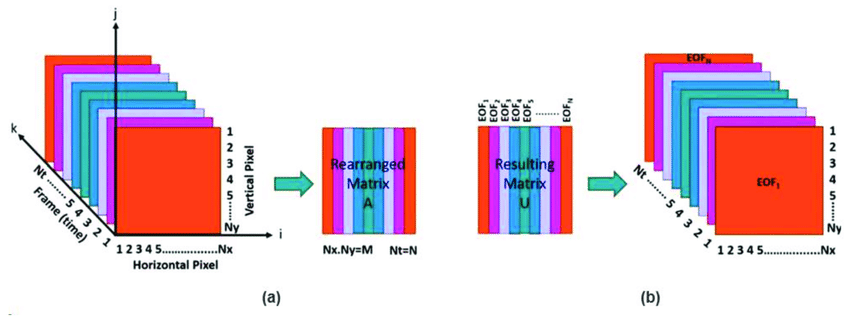
\includegraphics[width=.9 \columnwidth]{imglib/eof_matrix_decomp.png}
      {\tiny Source: \href{https://www.researchgate.net/publication/357212141_Latest_Advances_in_Common_Signal_Processing_of_Pulsed_Thermography_for_Enhanced_Detectability_A_Review/figures?lo=1}{researchgate}}
    \end{figure}

    \end{column}
    
  \end{columns}
\end{frame}

